% Revised October 30, 2026: BN-rounded MATLAB output
% Section 5 of SCOPE manuscript; inputs Figs/*.pdf
\section{Simulation study}
\label{sec:simul}

We investigate three questions: whether local coefficient energy improves
noise-calibrated SCOPE (Experiment~I), whether SURE can identify useful
neighborhoods without oracle information (Experiment~II), and how the
preselected methods compare with other implemented denoisers on independent
simulations (Experiment~III). Unlike a single-resolution comparison, the
present analysis covers three sample sizes and three signal strengths.
A representative $N=1024$, root-SNR $=5$ configuration is used for
condition-specific tables, whereas figures and normalized risk summaries
exhibit the dependence on sample size and signal strength. Complete numerical
results and implementation qualifications are organized in Supplementary
Section~S5.

\subsection{Design, noise calibration, and performance criteria}
\label{sec:simul-design}

The four Donoho--Johnstone test functions are Doppler, HeaviSine, Bumps,
and Blocks, sampled at $t_i=i/N$ with
$N\in\{512,1024,2048\}$. We observe
$y_i=f_N(t_i)+\varepsilon_i$, where the $\varepsilon_i$ are independent
$N(0,1)$ variables. Importantly, the \emph{executed MATLAB simulations}
set the root signal-to-noise ratio
\begin{eqnarray}
\rho_{\rm root} = \frac{\operatorname{sd}_N\{f_N(t_i)\}}{\sigma}
\in\{3,5,7\}, \qquad \sigma=1,
\label{eq:simul-root-snr}
\end{eqnarray}
by multiplying the uncentered test signal by
$\rho_{\rm root}/\operatorname{sd}_N(f_0)$, where
$\operatorname{sd}_N(f_0)=\{N^{-1}\sum_i(f_0(t_i)-\bar f_0)^2\}^{1/2}$.
The noise draws are \emph{not} rescaled individually. Thus $3,5,7$ are
standard-deviation ratios, not power SNR values
$N^{-1}\sum_i f_N(t_i)^2/\sigma^2$. This distinction matters because the
test functions need not have zero mean; all tables below report the
root-SNR convention of the supplied output.

We use periodized orthonormal wavelet transforms with Haar for Blocks,
Daubechies-3 (six taps) for Bumps, and Symmlet-4 (eight taps) for
Doppler and HeaviSine. For $N=2^J$, the scaling coefficients at $j_0=3$
(eight coefficients) remain unshrunk, whereas detail levels
$j=3,\ldots,J-1$ are estimated. Each realization uses
$\widehat\sigma=\operatorname{median}_{\ell}|d_{J-1,\ell}|/0.67448975$.
In accordance with Section~\ref{sec:calibration}, we use the direct
Gaussian null-risk calibration
$R_{F,r,k}(\lambda_{j,r}\widehat\sigma)=B_N/2^j$,
with the prespecified rounded budgets
$B_{512}=3.5$, $B_{1024}=5$, and $B_{2048}=7.5$. Here $B_N$ is
the expected retained standardized pure-noise energy per shrunk detail
level, not a per-coefficient threshold or an oracle risk choice. The
budget is shared across generators, exponents, and radii; the
corresponding inverse-risk scales are calibrated separately for each.
At $N=2048$, $B_N/2^3=0.9375$ at the coarsest shrunk level, so
that level is deliberately only weakly attenuated under pure noise.
The rounded budgets replace the former universal-threshold-based
numerical targets; the wavelet transforms and simulation design are
otherwise unchanged.

Each of the $4\times3\times3=36$ signal--strength--size settings uses
$M=1000$ Monte Carlo realizations for each experiment. Competing rules
within a condition share the same Gaussian noise realizations; Experiment~III
uses new random streams, separate from those of Experiments~I--II.
For procedure $m$, let $L_{m,s,q,N}^{(\nu)}$ denote the average squared
reconstruction error in replication $\nu$. We report
\begin{eqnarray}
\operatorname{AMSE}_{m,s,q,N}
 &=&\frac1M\sum_{\nu=1}^M L_{m,s,q,N}^{(\nu)},\qquad
L_{m,s,q,N}^{(\nu)}=\frac1N\sum_{i=1}^N
\{\widehat f_{m}^{(\nu)}(t_i)-f_N(t_i)\}^2.
\label{eq:simul-plan-amse}
\end{eqnarray}
True signals are used exclusively to \emph{assess} estimation error, never
to select the tuning parameters of a particular reconstruction. We use
paired replication-level MSE differences for inferential comparisons.
For comparisons across signals with unequal baseline difficulty, define
\begin{eqnarray}
Q_N(m)=\frac1{12}\sum_{s\in\mathcal D}\sum_{q\in\{3,5,7\}}
\frac{\operatorname{AMSE}_{m,s,q,N}}
{\operatorname{AMSE}_{{\rm Hard},s,q,N}},
\qquad \mathcal D=\{\text{Doppler, HeaviSine, Bumps, Blocks}\}.
\label{eq:simul-overall-score}
\end{eqnarray}
Here ``Hard'' is universal hard thresholding with
$\widehat\sigma\sqrt{2\log N}$. Hence $Q_N$ is the equal-weighted mean of
12 \emph{conditionwise normalized} AMSEs, not the ratio of pooled AMSEs
and not an oracle criterion. When an across-size descriptor is useful,
we use $Q_{\rm all}(m)=\{Q_{512}(m)+Q_{1024}(m)+Q_{2048}(m)\}/3$;
raw MSE values are never averaged across distinct sample sizes.

\subsection{Experiment I: fixed calibration and neighborhood radius}
\label{sec:simul-fixed}

For each of six generating distributions (Normal, logistic, Laplace,
hyperbolic secant, Uniform, and Cauchy), we fix $k=5$ and examine
$r=0,1,2,3$. Each radius receives its own scale
$\lambda_{j,r}^{\rm fix}(F,5,N)=
R_{F,r,5}^{-1}(B_N/2^j)/\widehat\sigma$, obtained from the
Gaussian null-risk integral in Section~\ref{sec:calibration}; thus
comparison across radii is not confounded by using the same uncalibrated
scale. No SURE optimization or use of the clean signal is involved.
Table~\ref{tab:e1-normal} gives the Normal-generator AMSEs for
$N=1024$ and root SNR $5$.

\begin{table}[tbp]
\centering\small
\caption{Experiment I: AMSE for fixed Normal-generator SCOPE ($r=0$) and N-SCOPE ($r=1,2,3$), $N=1024$, root SNR $=5$, $k=5$, $B_N=5$, and $M=1000$. All radii use separately calibrated Gaussian null-risk constants. Bold indicates the smallest AMSE within a signal.}
\label{tab:e1-normal}
\setlength{\tabcolsep}{5pt}
\begin{tabular}{lcccc}
\toprule
Signal & $r=0$ & $r=1$ & $r=2$ & $r=3$ \\
\midrule
Doppler & 0.1610 & 0.1327 & \textbf{0.1273} & 0.1285 \\
HeaviSine & \textbf{0.0690} & 0.0730 & 0.0793 & 0.0847 \\
Bumps & 0.3137 & \textbf{0.2356} & 0.2798 & 0.3220 \\
Blocks & \textbf{0.1239} & 0.2023 & 0.2587 & 0.3025 \\
\bottomrule
\end{tabular}
\end{table}

The effect of neighborhood energy is strongly morphology dependent.
At the representative setting, the percentage reductions in
Normal-generator AMSE on moving from $r=0$ to $r=1$ are
+17.6\%, +24.9\%, -5.9\%, and -63.2\%
for Doppler, Bumps, HeaviSine, and Blocks, respectively. For Doppler, the best fixed radius among
$r=0,1,2,3$ is $r=2$, whereas Bumps favors $r=1$.
For Blocks, a positive radius damages isolated wavelet features near
jumps, despite the common null-risk calibration. This distinction is
structural: N-SCOPE alters the attenuation of the \emph{central}
coefficient based on overlapping neighborhood energy; it does not
assign one factor to an entire block.

Figure~\ref{fig:e1-cdf-gain} compares the effect of $r=1$ over all
six generators, averaging percentage AMSE changes equally over the three
root-SNR values at $N=1024$. The sample-size robustness is shown in
Figure~\ref{fig:e1-size-snr}, with separate curves for each root SNR.
Each curve compares the \emph{fixed} Normal N-SCOPE rule at $r=1$ against
the fixed Normal $r=0$ rule; no radius is selected retrospectively.
The signs and magnitudes of these gains vary by signal and, particularly
for Blocks, by sample size and signal strength. Therefore neighborhoods
cannot be defended as uniformly beneficial.

\begin{figure}[tbp]
\centering
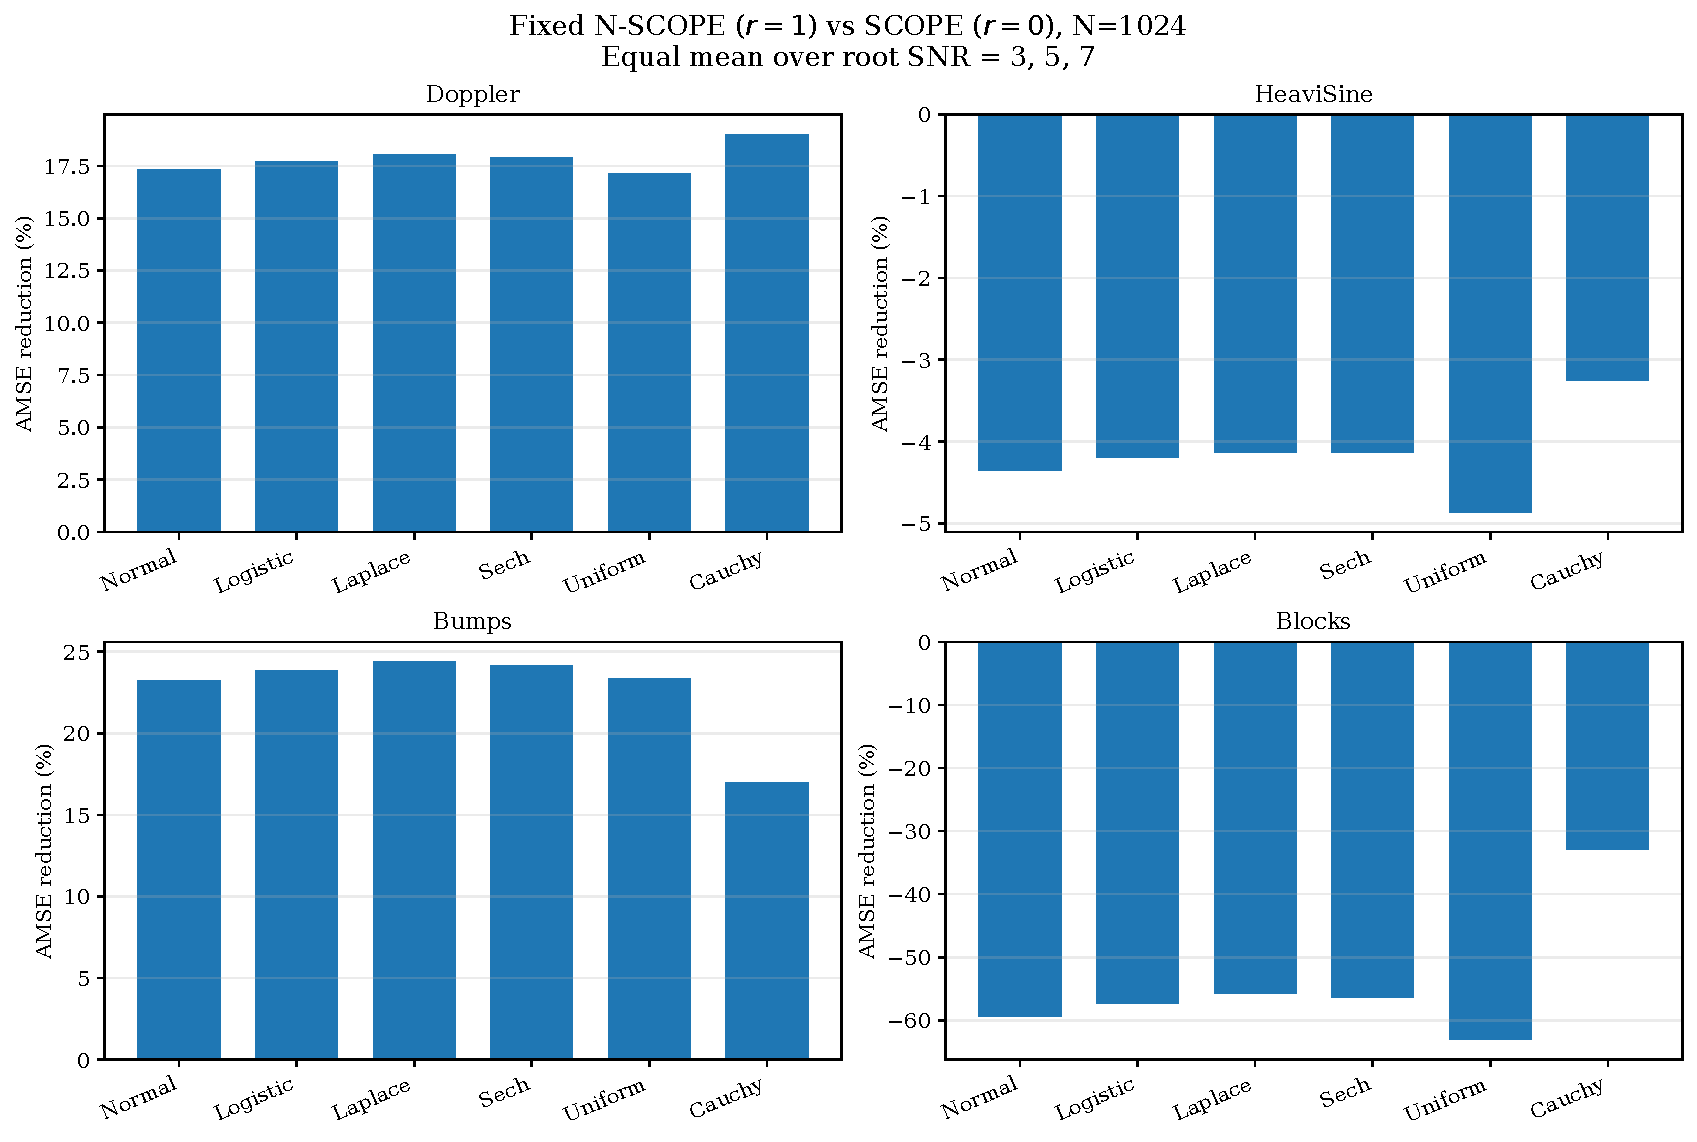
\includegraphics[width=.93\linewidth]{Figs/E1_gain_CDF_N1024.pdf}
\caption{Experiment I: reduction in AMSE (%) on moving from fixed
$r=0$ to fixed $r=1$ at $N=1024$, averaged \emph{equally across}
root SNR $3,5,7$ for each test signal and centered-CDF generator.
Positive values favor N-SCOPE. The comparison is separately calibrated
at the same null-risk target for each radius.}
\label{fig:e1-cdf-gain}
\end{figure}

\begin{figure}[tbp]
\centering
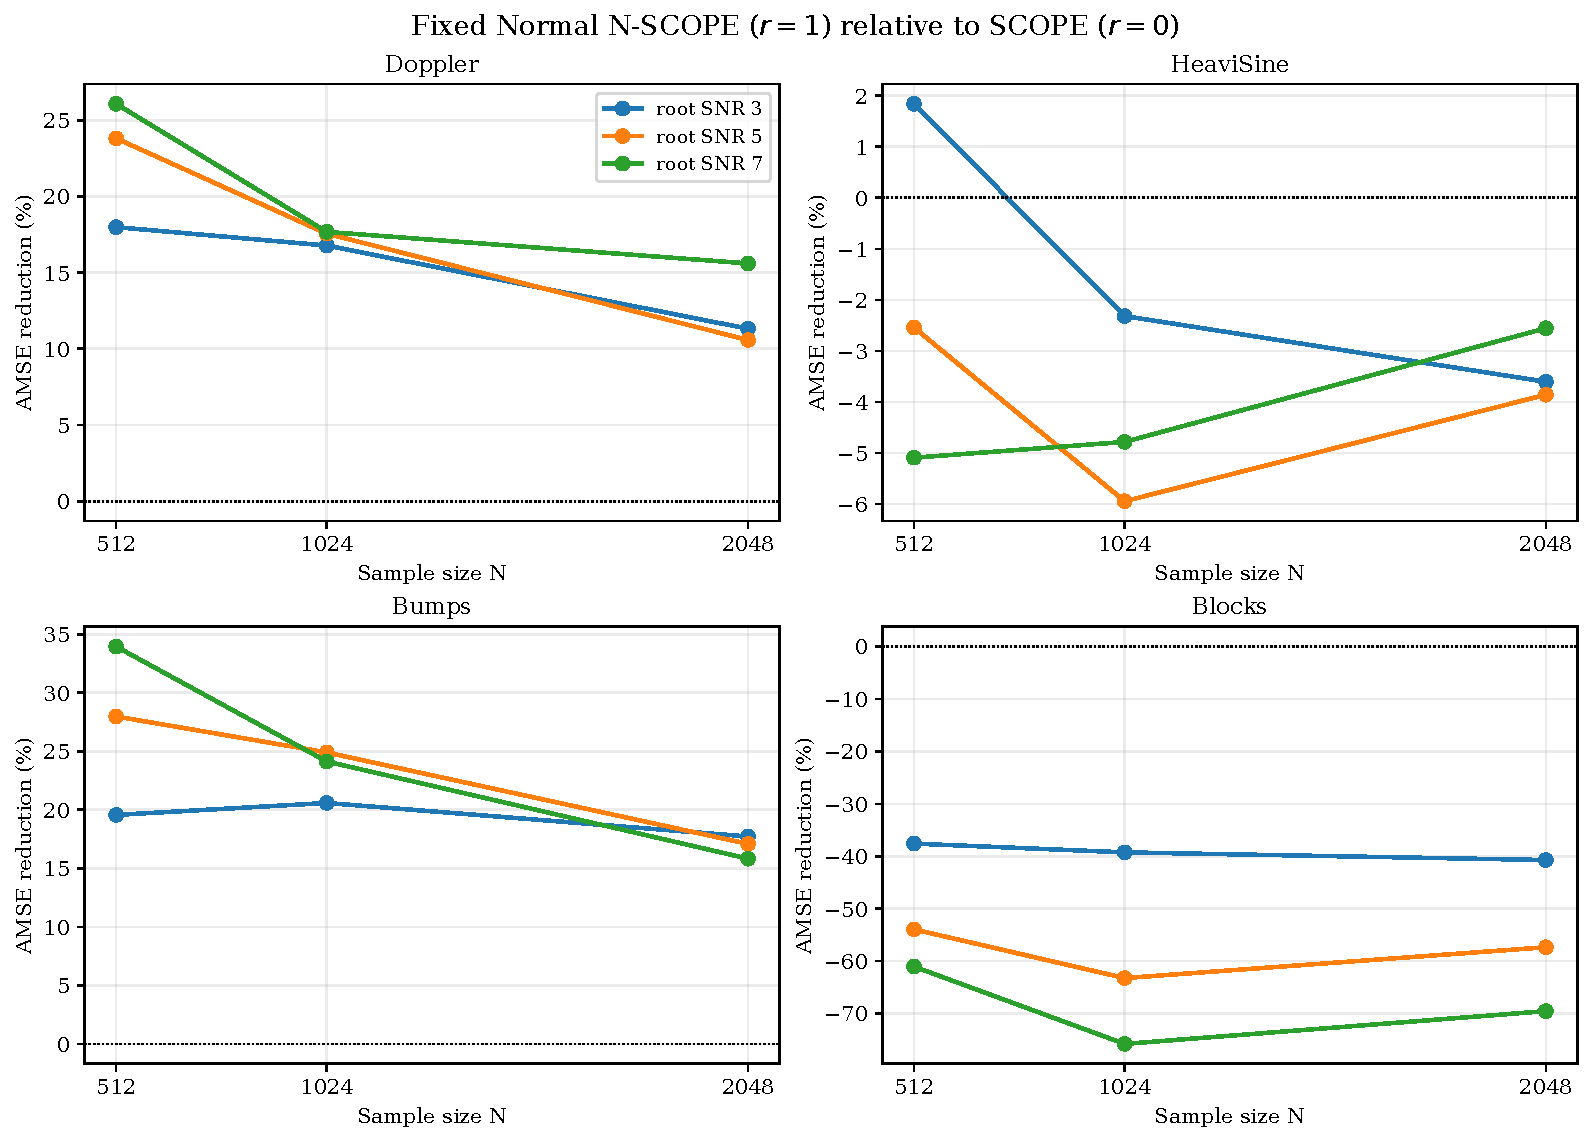
\includegraphics[width=.95\linewidth]{Figs/E1_sensitivity_N_rootSNR.pdf}
\caption{Experiment I: sample-size and root-SNR sensitivity of the
percentage AMSE reduction of fixed Normal-generator N-SCOPE ($r=1$)
relative to coefficientwise SCOPE ($r=0$), across $N=512,1024,2048$.
Each point is based on $M=1000$ paired realizations; positive values
indicate improvement.}
\label{fig:e1-size-snr}
\end{figure}

\subsection{Experiment II: data-adaptive attenuation and neighborhoods}
\label{sec:simul-sure}

For each fixed generator $F$, SCOPE SURE selects $(k,b)$ with $r=0$
from 15 candidates, whereas N-SCOPE SURE selects $(k,r,b)$ from 60
candidates, using $k\in\{3,5,7\}$,
$r\in\{0,1,2,3\}$, and
$b\in\{0.65,0.80,1,1.20,1.50\}$. The candidate scale is
$\lambda_{j,r}(F,k,b)=
b\,R_{F,r,k}^{-1}(B_N/2^j)/\widehat\sigma$.
The plug-in SURE score uses the derivative of the \emph{central}
coefficient estimator, including the dependence of its local RMS on
that coefficient. The estimate $\widehat\sigma$ is held fixed for the
derivative. Selection minimizes the score \emph{globally over the
shrunk detail levels} in each noisy realization, while local energies
still depend on coefficient position. Neither the generator nor the true
signal is selected from the observed signal by this search: generator
families are compared externally, and clean coefficients appear only
when evaluating AMSE. We do not claim exact unbiasedness for plug-in,
after-selection SURE.

\begin{table}[tbp]
\centering\small
\caption{Experiment II: paired AMSE of four Normal-generator procedures at $N=1024$, root SNR $=5$, and $B_N=5$ ($M=1000$). Fixed rules use $(k,b)=(5,1)$; SURE selects $(k,b)$ at $r=0$ or $(k,r,b)$ with $r\in\{0,1,2,3\}$. Bold indicates the smallest observed AMSE for each signal (ties shown).}
\label{tab:e2-normal}
\setlength{\tabcolsep}{5pt}
\begin{tabular}{lcccc}
\toprule
Signal & Fixed SCOPE & Fixed N-SCOPE & SCOPE SURE & N-SCOPE SURE \\
\midrule
Doppler & 0.1610 & 0.1327 & 0.1638 & \textbf{0.1242} \\
HeaviSine & 0.0690 & 0.0730 & \textbf{0.0578} & 0.0601 \\
Bumps & 0.3137 & 0.2356 & 0.2915 & \textbf{0.2347} \\
Blocks & 0.1239 & 0.2023 & \textbf{0.1210} & \textbf{0.1210} \\
\bottomrule
\end{tabular}
\end{table}

For the Normal generator at $N=1024$, root SNR $5$, the relative
reduction of N-SCOPE SURE versus coefficientwise SCOPE SURE is
+24.2\%, +19.5\%, -3.9\%, and +0.0\%
for Doppler, Bumps, HeaviSine, and Blocks, respectively.
As predicted by the radius experiment, adaptive neighborhoods improve
recovery of locally coherent Doppler and Bumps structures. For
HeaviSine, most of the benefit comes from adjusting the attenuation
shape and scale; the extra neighborhood search gives little additional
benefit and can be mildly unfavorable. For Blocks, the two SURE
procedures are close because radius zero remains available in the
larger candidate set. Nesting ensures a no-greater \emph{minimum
estimated SURE}, not necessarily a smaller true AMSE.

Table~\ref{tab:e2-cdf-ranking} places these condition-specific
comparisons in perspective, using $Q_N$ at each sample size and retaining
both Normal and logistic generators. In particular, the Normal-generator
improvement in $Q_N$ from SCOPE SURE to N-SCOPE SURE is
10.4\%, 9.7\%, and 9.7\% at $N=512,1024,2048$, respectively.
Across the three sample sizes, $Q_{\rm all}$ declines from $0.7045$ to $0.6347$, a relative reduction of $9.9\%$. These figures are
\emph{relative reductions of normalized risks}, not percentage points.
The complete six-generator scores are supplied in Section~S5.

\begin{table}[tbp]
\centering\small
\caption{Experiment II: macro-average normalized AMSE $Q_N$ (relative to universal hard thresholding), averaged equally over the four signals and root SNR $3,5,7$, separately for each sample size, using rounded $B_N$. Lower is better. These are descriptive normalized risks, not pooled raw MSEs.}
\label{tab:e2-cdf-ranking}
\setlength{\tabcolsep}{5pt}
\begin{tabular}{llcccc}
\toprule
$N$ & Generator & Fixed SCOPE & Fixed N-SCOPE & SCOPE SURE & N-SCOPE SURE \\
\midrule
512 & Normal & 0.7105 & 0.7377 & 0.6816 & 0.6106 \\
512 & Logistic & 0.7210 & 0.7467 & 0.6863 & 0.6182 \\
1024 & Normal & 0.7398 & 0.8069 & 0.7004 & 0.6327 \\
1024 & Logistic & 0.7524 & 0.8173 & 0.7090 & 0.6424 \\
2048 & Normal & 0.7995 & 0.8859 & 0.7315 & 0.6609 \\
2048 & Logistic & 0.8093 & 0.8945 & 0.7438 & 0.6721 \\
\bottomrule
\end{tabular}
\end{table}

The selected radius provides an interpretation of the observed
adaptation. Figure~\ref{fig:e2-radius-selection} shows the
Normal-generator selection frequencies at $N=1024$, pooled equally
over the three root-SNR settings. It is particularly informative
whether $r=0$ is favored for Blocks and larger values are favored for
Doppler. Full tables in Section~S5 also show how radius frequencies
change with sample size, generator, and SNR. Selection of $k$ and $b$
is not universal either, so the advantage of N-SCOPE SURE should be
attributed to joint attenuation-and-neighborhood adaptation rather
than to a single preferred radius.

\begin{figure}[tbp]
\centering
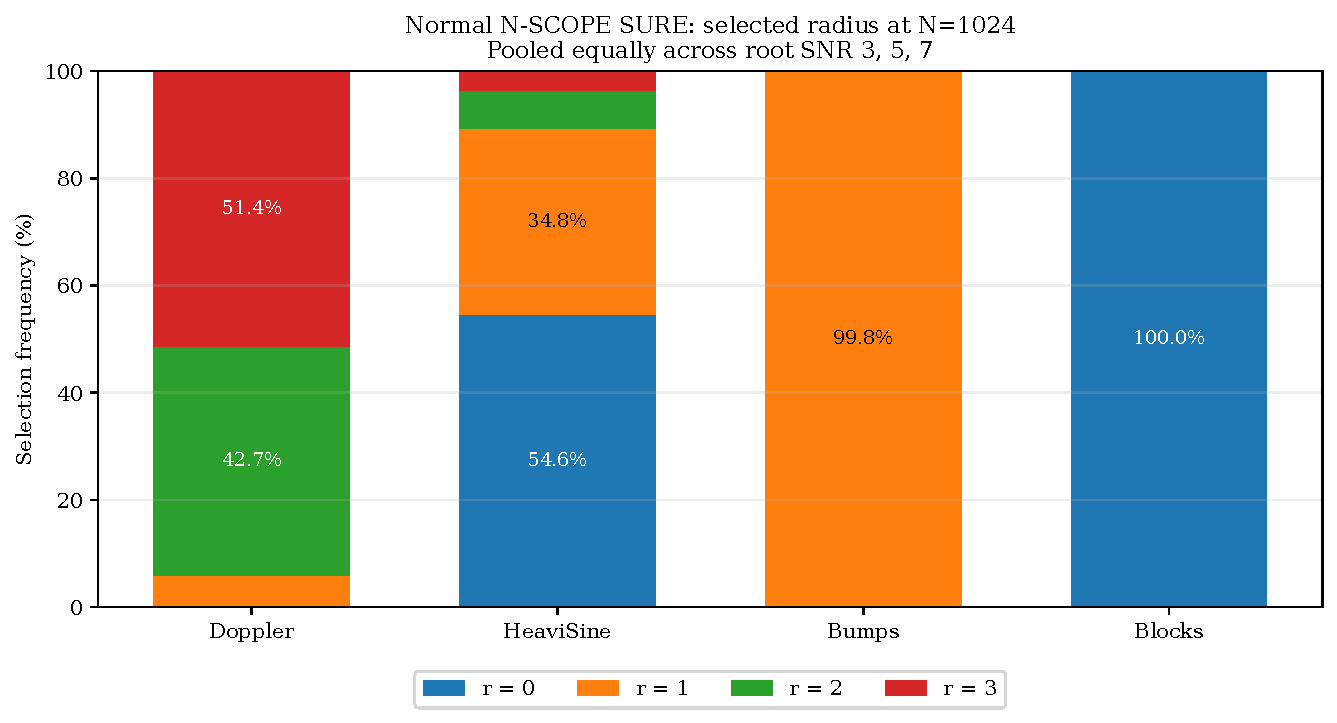
\includegraphics[width=.90\linewidth]{Figs/E2_selected_radius_Normal_N1024.pdf}
\caption{Experiment II: Normal-generator N-SCOPE SURE selection
frequencies for $r=0,1,2,3$ at $N=1024$, pooled equally over
root SNR $3,5,7$ ($M=1000$ for each signal--SNR condition).
A separate radius is chosen for each noisy realization, not each
wavelet coefficient.}
\label{fig:e2-radius-selection}
\end{figure}

\subsection{Experiment III: independently simulated comparator study}
\label{sec:simul-competitors}

We next compare four recipes frozen before a new Monte Carlo experiment:
Normal-generator fixed SCOPE $(k,r,b)=(5,0,1)$, Normal-generator
fixed N-SCOPE $(5,1,1)$, Normal SCOPE SURE (radius zero), and Normal
N-SCOPE SURE (free radius). All four use the same rounded-$B_N$ noise-energy calibration
as in Experiments~I--II. Independent random streams are used at each
$N$; within each simulated condition, all procedures receive the same
noise realization. The additional 20 codes represent a range of
empirical Bayes, smooth, thresholding, neighborhood, and block-inspired
approaches. These are comparisons among \emph{executed MATLAB
implementations}, and are not all verified implementations of the
named published methods. In particular, the one-dimensional hidden
Markov tree (HMT) code is explicitly a \emph{provisional proxy} and
must not be described as a validated implementation of published HMT
wavelet denoising. Similarly, several image-domain methods were
adapted to one dimension; algorithmic fidelity and original parameter
conventions still require audit.


%% Experiment III. Source: SCOPE_Exp123_results_BNrounded.zip, Exp3_N1024_M1000/Experiment3_AMSE_all.csv, M=1000
\begin{landscape}
\begin{center}
\begingroup
\singlespacing
\setlength{\tabcolsep}{2.35pt}
\renewcommand{\arraystretch}{1.0}
\fontsize{7}{8}\selectfont
\captionsetup{font=footnotesize,skip=5pt}
\captionof{table}{Experiment III: average mean squared error (AMSE) for all 26 executed MATLAB procedures at $N=1024$ and root SNR $3,5,7$. Within each SNR, the four columns correspond to Doppler (D), HeaviSine (H), Bumps (Bu), and Blocks (Bl). Each entry averages $M=1000$ paired Monte Carlo replications under the rounded-$B_N$ calibration. BAMS uses the author's parameters and the correct decomposition depth; CYV Context uses the updated 1D context model. Bold indicates the lowest AMSE among the 26 executed implementations (including provisional proxies).}
\label{tab:e3-all-methods}
\medskip
\begin{tabular}{@{}r p{7.55cm}*{12}{r}@{}}
\toprule
& & \multicolumn{4}{c}{Root SNR $3$} & \multicolumn{4}{c}{Root SNR $5$} & \multicolumn{4}{c}{Root SNR $7$} \\
\cmidrule(lr){3-6}\cmidrule(lr){7-10}\cmidrule(l){11-14}
No. & Procedure and source & D & H & Bu & Bl & D & H & Bu & Bl & D & H & Bu & Bl \\
\midrule
\multicolumn{14}{@{}l}{\emph{SCOPE procedures (prespecified Normal generator)}}\\
1 & Fixed SCOPE (Normal; $r=0$) & 0.1354 & 0.0626 & 0.2835 & 0.1595 & 0.1617 & 0.0693 & 0.3138 & 0.1250 & 0.1805 & 0.0774 & 0.3204 & 0.1050 \\
2 & Fixed N-SCOPE (Normal; $r=1$) & 0.1129 & 0.0641 & 0.2254 & 0.2215 & 0.1331 & 0.0733 & 0.2348 & 0.2028 & 0.1491 & 0.0808 & \textbf{0.2427} & 0.1842 \\
3 & SCOPE SURE (Normal; $r=0$) & 0.1396 & 0.0506 & 0.2738 & 0.1584 & 0.1646 & \textbf{0.0573} & 0.2909 & 0.1218 & 0.1821 & 0.0688 & 0.2946 & 0.1037 \\
4 & N-SCOPE SURE (Normal) & \textbf{0.1033} & 0.0510 & \textbf{0.2242} & 0.1584 & \textbf{0.1246} & 0.0596 & \textbf{0.2342} & 0.1218 & 0.1384 & 0.0709 & 0.2457 & 0.1037 \\
\addlinespace[2pt]
\multicolumn{14}{@{}l}{\emph{Literature-based MATLAB implementations (references identify target methods)}}\\
5 & BAMS (author parameters) \citep{VidakovicRuggeri2001BAMS}$^{\ast}$ & 0.1356 & 0.0556 & 0.2890 & 0.1546 & 0.1649 & 0.0586 & 0.3326 & 0.1197 & 0.1855 & \textbf{0.0657} & 0.3522 & 0.0975 \\
6 & EBayesThresh posterior median \citep{JohnstoneSilverman2005EBayes}$^{\dagger}$ & 0.1441 & 0.0511 & 0.2965 & 0.1662 & 0.1779 & 0.0606 & 0.3168 & 0.1275 & 0.1974 & 0.0724 & 0.3239 & 0.1184 \\
7 & Raised-cosine Bayes \citep{ReinaSousa2026RaisedCosine}$^{\dagger}$ & 0.1518 & 0.0503 & 0.3275 & 0.1682 & 0.2036 & 0.0624 & 0.3768 & 0.1276 & 0.2722 & 0.0713 & 0.3980 & 0.1174 \\
8 & Epanechnikov Bayes (1D) \citep{BarriosSousa2025Epanechnikov}$^{\dagger}$ & 0.1466 & \textbf{0.0467} & 0.3679 & 0.2078 & 0.1872 & 0.0596 & 0.5086 & 0.2028 & 0.2185 & 0.0736 & 0.6711 & 0.2076 \\
9 & Smooth SCAD (stabilized) \citep{KulkarniEtAl2026SmoothSCAD}$^{\dagger}$ & 0.1451 & 0.0681 & 0.3121 & 0.1564 & 0.1731 & 0.0667 & 0.3324 & 0.1151 & 0.1885 & 0.0724 & 0.3328 & 0.0966 \\
10 & SureShrink (hybrid) \citep{DonohoJohnstone1995SureShrink}$^{\dagger}$ & 0.2024 & 0.0540 & 0.3614 & 0.3270 & 0.2283 & 0.0695 & 0.4321 & 0.2854 & 0.2900 & 0.0826 & 0.4557 & 0.2157 \\
11 & FDR ($q=0.05$) \citep{AbramovichEtAl2006FDR}$^{\dagger}$ & 0.1777 & 0.0997 & 0.3538 & 0.1784 & 0.2059 & 0.0859 & 0.3650 & 0.1304 & 0.2159 & 0.0822 & 0.3547 & 0.1145 \\
12 & Empirical Bayes block (1D) \citep{AbramovichBesbeasSapatinas2002BlockEB}$^{\ddagger}$ & 0.1480 & 0.0498 & 0.3664 & 0.3482 & 0.2061 & 0.0681 & 0.4142 & 0.3729 & 0.2399 & 0.0904 & 0.4267 & 0.3533 \\
13 & BayesShrink (1D) \citep{ChangYuVetterli2000BayesShrink}$^{\dagger}$ & 0.1693 & 0.0488 & 0.3558 & 0.2410 & 0.2347 & 0.0661 & 0.4283 & 0.3167 & 0.2822 & 0.0867 & 0.4999 & 0.4164 \\
14 & NeighCoeff \citep{CaiSilverman2001Neigh}$^{\dagger}$ & 0.1326 & 0.0748 & 0.3174 & 0.3401 & 0.1688 & 0.0809 & 0.2974 & 0.3088 & 0.1867 & 0.0864 & 0.2864 & 0.2579 \\
15 & NeighShrink--SURE (1D) \citep{ZhouCheng2008NeighShrinkSURE}$^{\dagger}$ & 0.1068 & 0.0592 & 0.2419 & 0.2326 & 0.1253 & 0.0723 & 0.2427 & 0.2184 & \textbf{0.1374} & 0.0835 & 0.2474 & 0.2040 \\
16 & SURE-LET (1D two-term) \citep{BluLuisier2007SURELET}$^{\ddagger}$ & 0.1559 & 0.0825 & 0.2901 & 0.1781 & 0.1833 & 0.0866 & 0.3179 & 0.1553 & 0.2024 & 0.0949 & 0.3314 & 0.1424 \\
17 & Sendur--Selesnick BiShrink (1D) \citep{SendurSelesnick2002BiShrink}$^{\dagger}$ & 0.1096 & 0.0748 & 0.2636 & 0.1921 & 0.1254 & 0.0865 & 0.2828 & 0.2061 & 0.1377 & 0.0949 & 0.2971 & 0.2215 \\
18 & NeighBlock \citep{CaiSilverman2001Neigh}$^{\dagger}$ & 0.1218 & 0.0859 & 0.4217 & 0.4680 & 0.1540 & 0.1063 & 0.4021 & 0.4664 & 0.1752 & 0.1139 & 0.3800 & 0.4008 \\
19 & SureBlock (hybrid) \citep{CaiZhou2009SureBlock}$^{\ddagger}$ & 0.1621 & 0.0513 & 0.3013 & 0.2537 & 0.1822 & 0.0623 & 0.3308 & 0.1713 & 0.2217 & 0.0761 & 0.3336 & 0.1365 \\
20 & BlockJS \citep{Cai1999BlockJS}$^{\dagger}$ & 0.1380 & 0.0843 & 0.5599 & 0.4981 & 0.1755 & 0.1177 & 0.5369 & 0.5244 & 0.1967 & 0.1288 & 0.4987 & 0.4534 \\
21 & Jeffreys-prior EB (1D) \citep{FigueiredoNowak2001Jeffreys}$^{\ddagger}$ & 0.1730 & 0.1132 & 0.2986 & 0.1711 & 0.1916 & 0.1158 & 0.3168 & 0.1543 & 0.2051 & 0.1191 & 0.3230 & 0.1445 \\
22 & Local Bayesian Wiener (1D) \citep{MihcakEtAl1999LocalWiener}$^{\dagger}$ & 0.1617 & 0.1295 & 0.3120 & 0.2973 & 0.1732 & 0.1429 & 0.3342 & 0.3185 & 0.1818 & 0.1501 & 0.3472 & 0.3239 \\
23 & CYV Context (1D orthonormal) \citep{ChangYuVetterli2000Context}$^{\ddagger}$ & 0.1391 & 0.0591 & 0.2687 & 0.1940 & 0.1619 & 0.0753 & 0.2829 & 0.1983 & 0.1796 & 0.0918 & 0.2914 & 0.2055 \\
24 & Hidden Markov tree (1D EM) \citep{CrouseNowakBaraniuk1998HMT}$^{\ddagger}$ & 0.1189 & 0.0607 & 0.2385 & \textbf{0.1012} & 0.1447 & 0.0598 & 0.2413 & \textbf{0.0779} & 0.1639 & 0.0730 & 0.2589 & \textbf{0.0718} \\
\addlinespace[2pt]
\multicolumn{14}{@{}l}{\emph{Universal-threshold references}}\\
25 & Universal hard threshold \citep{DonohoJohnstone1994} & 0.1946 & 0.0989 & 0.4479 & 0.2275 & 0.2376 & 0.0919 & 0.4793 & 0.1460 & 0.2420 & 0.0829 & 0.4875 & 0.1124 \\
26 & Universal soft threshold \citep{DonohoJohnstone1994} & 0.4622 & 0.1202 & 1.2951 & 0.6863 & 0.6525 & 0.2033 & 1.7067 & 0.8250 & 0.7825 & 0.2484 & 1.9976 & 0.8654 \\
\bottomrule
\end{tabular}
\par\smallskip
\begin{minipage}{\linewidth}
\raggedright\fontsize{7}{8}\selectfont
$^\ast$ Author-parameter BAMS: $C_{\rm scale}=2$, $\gamma=2$, decomposition depth $J-3$, and $\tau_j=\tau_u\sqrt{j}$. $^\dagger$ Audit pending; may be adapted, stabilized, or hybrid.
$^\ddagger$ Provisional proxy or 1D adaptation, not established as the original published algorithm; the CYV implementation uses four lateral neighbors, a parent context, least-squares weights, and context-grouped soft thresholds.
Citations identify originating publications, not verified numerical reproductions.
Root SNR $=\operatorname{SD}(f)/\sigma$ with $\sigma=1$ (not power SNR).
Matched noise is used across procedures within each replication.
See Supplement Section~S5 for the implementation inventory and other sizes.
\end{minipage}
\endgroup
\end{center}
\end{landscape}


Table~\ref{tab:e3-all-methods} reports all 26 procedures at
$N=1024$ for each of the three root-SNR values, with the corrected
BAMS and CYV Context implementations. The BAMS implementation uses
the author-specified constants $C_{\rm scale}=2$ and $\gamma=2$,
seven decomposition steps at $N=1024$ (that is, $J-3$), and
$\tau_j=\tau_u\sqrt{j}$. The CYV code uses a one-dimensional
orthonormal-wavelet adaptation of context regression and grouping:
four lateral neighbors and a parent coefficient determine the context,
and coefficients with nearby context values supply local variance
estimates for adaptive soft thresholds. Neither implementation is
tuned against the simulated truth.

Normal N-SCOPE SURE yields the smallest observed Doppler AMSE at
root SNR $3$ and $5$ (0.1033 and 0.1246, respectively); the 1D
NeighShrink--SURE adaptation is narrowly lower at root SNR $7$
(0.1374 versus 0.1384). For Bumps, N-SCOPE SURE is best at root SNR
$3$ and $5$ (0.2242 and 0.2342), while fixed $r=1$ N-SCOPE is
slightly better at root SNR $7$ (0.2427 versus 0.2457).
For HeaviSine, the Epanechnikov-inspired method has the smallest
AMSE at root SNR $3$ (0.0467), coefficientwise SCOPE SURE at root
SNR $5$ (0.0573), and \emph{the corrected author-parameter BAMS}
at root SNR $7$ (0.0657, compared with 0.0688 for SCOPE SURE).
BAMS also performs competitively for Blocks (AMSE 0.1546, 0.1197,
and 0.0975 at root SNR $3,5,7$, respectively), although the
provisional HMT code is numerically lowest in all three Blocks
conditions (0.1012, 0.0779, and 0.0718).

The revised CYV Context method improves substantially over the
previous local-energy proxy for Bumps and Blocks but is not the
minimum-AMSE procedure in any of the 12 displayed conditions. At
$N=1024$, the experiment-specific normalized aggregate scores are
$Q_{1024}=0.6022$ for the \emph{unverified} HMT proxy, $0.6327$
for Normal N-SCOPE SURE, $0.7002$ for Normal SCOPE SURE,
$0.7149$ for BAMS, and $0.8740$ for CYV Context. The HMT figure
must not be interpreted as evidence that the original published
HMT algorithm outperforms N-SCOPE. These are rankings of the
\emph{executed implementations}, not verified rankings of the
original methods. Figure~\ref{fig:e3-profile} includes the corrected
BAMS and CYV results; Supplementary Section~S5 gives all 26
normalized scores separately for $N=512,1024,2048$.

\begin{figure}[tbp]
\centering
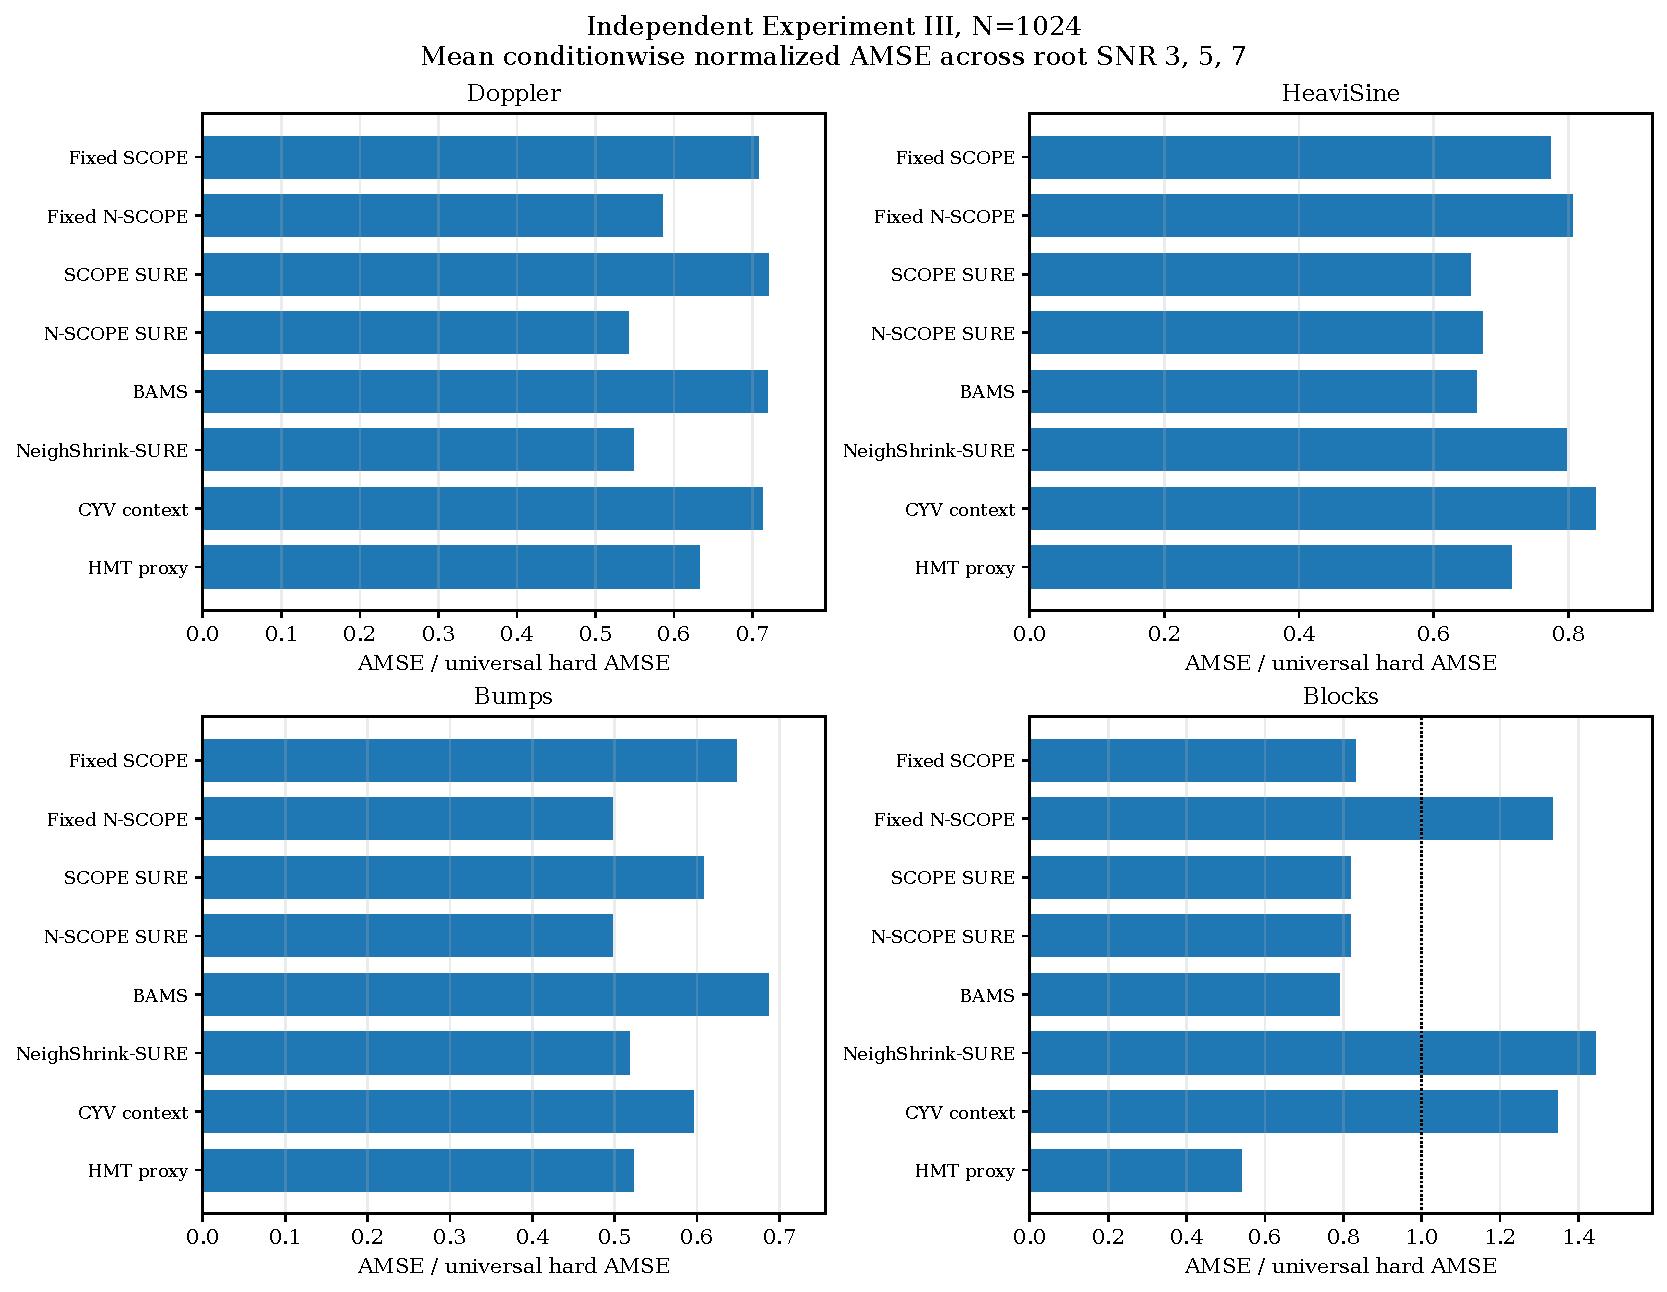
\includegraphics[width=.95\linewidth]{Figs/E3_signal_profile_Normal_N1024.pdf}
\caption{Experiment III: signalwise mean AMSE relative to universal
hard thresholding at $N=1024$, averaged equally over root SNR
$3,5,7$. The figure includes the corrected author-parameter BAMS
and the revised one-dimensional CYV Context implementation. The
HMT result represents an unverified one-dimensional proxy, not
a reproduction of the published HMT algorithm.}
\label{fig:e3-profile}
\end{figure}

\subsection{Interpretation and limitations}
\label{sec:simul-discussion}

The three experiments yield a consistent qualitative conclusion:
neighboring detail-coefficient energy is valuable for clustered wavelet
features, but can be detrimental for isolated coefficients. By
allowing $r=0$, the SURE search can largely avoid the Blocks failure
mode of a fixed positive radius, while retaining benefits for Doppler
and Bumps. However, a larger parameter search has its own selection
variability, and no uniform risk improvement is implied.
The rounded $B_N$ budgets are prespecified approximations to the
universal-threshold-anchored null-risk allocations, not estimates of
risk-optimal scales. Their per-level allocation becomes permissive at
$N=2048$ and $j=3$, where $B_N/2^3=0.9375$. Also, the plug-in SURE derivative neglects the
sampling variation of $\widehat\sigma$; its formal unbiasedness does
not extend automatically to the complete selected estimator.
Finally, rankings in Experiment~III are conditional on the exact
comparator codes and their adaptation to one-dimensional, periodized,
orthonormal wavelets.
The BAMS depth error and the earlier CYV context proxy have been
corrected in these tables; these corrections do not constitute
independent validation of every other competitor. Until every literature method has been audited,
the safe inference is that N-SCOPE is competitive among the tested
implementations, \emph{not} that it dominates all established
wavelet denoisers. Reporting every sample size and signal condition,
rather than the most favorable one, is essential for that conclusion.
